% -*- compile-command: "cd ../ && make" -*-
\eocesolch{Probability}
\begin{multicols}{2}

% 1

\eocesol{(a)~False. These are independent trials.
(b)~False. There are red face cards.
(c)~True. A card cannot be both a face card and an ace.}

% 3

\eocesol{(a)~10 tosses. Fewer tosses mean more variability in the sample fraction of heads,
meaning there's a better chance of getting at least 60\% heads.
(b)~100 tosses. More flips means the observed proportion of heads would often be
closer to the average, 0.50, and therefore also above 0.40.
(c)~100 tosses. With more flips, the observed proportion of heads would often be
closer to the average, 0.50.
(d)~10 tosses. Fewer flips would increase variability in the fraction of tosses
that are heads.}

% 5

\eocesol{(a)~$0.5^{10}$ = 0.00098.
(b)~$0.5^{10}$ = 0.00098.
(c)~$P$(at least one tails) = $1 - P$(no tails) = $1 - (0.5^{10}) \approx 1 - 0.001 = 0.999$.}

% 7

\eocesol{(a)~No, there are voters who are both independent and swing voters. \\
(b) \\
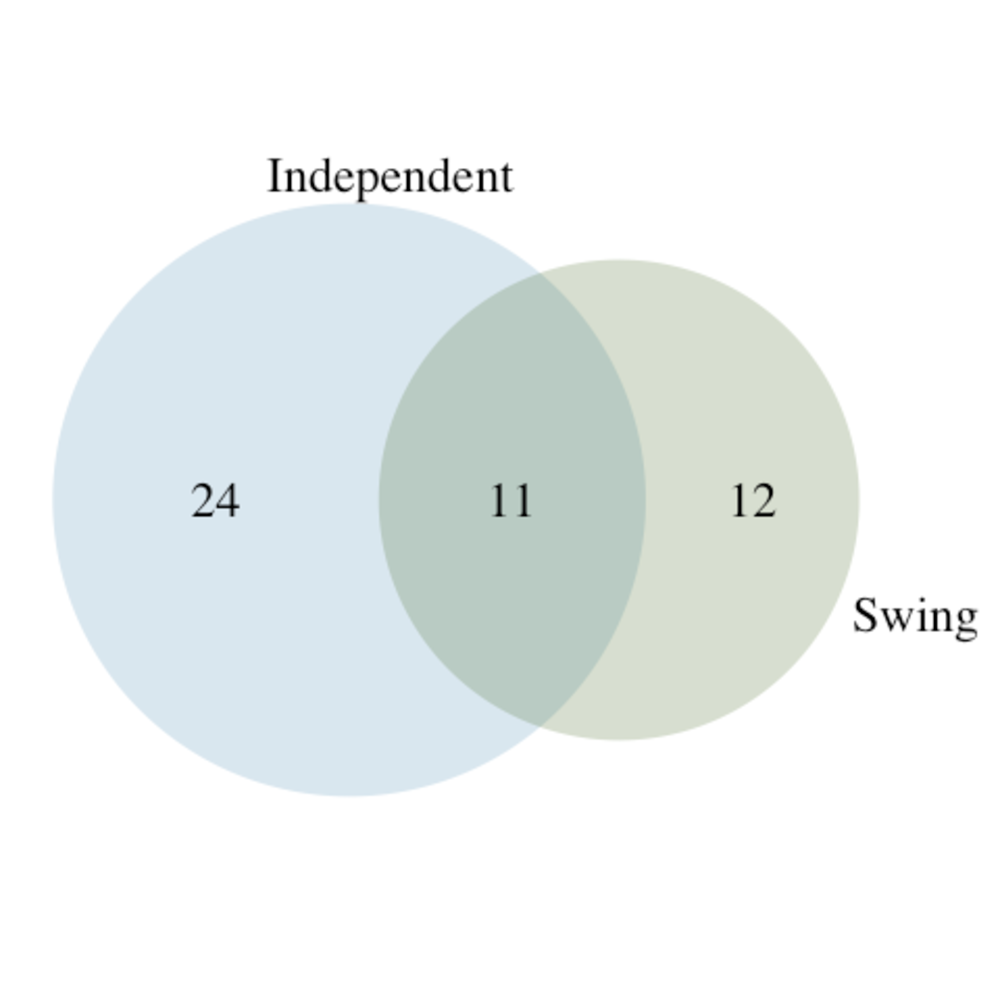
\includegraphics[width=40mm]{ch_probability/figures/eoce/swing_voters/swing_voters.pdf} \\
(c)~Each Independent voter is either a swing voter or not. Since 35\% of voters
are Independents and 11\% are both Independent and swing voters, the other 24\%
must not be swing voters.
(d)~0.47.
(e)~0.53.
(f)~P(Independent) $\times$ P(swing) = $0.35\times0.23 = 0.08$, which
does not equal P(Independent and swing) = 0.11, so the events are dependent.}

% 9

\eocesol{(a)~If the class is not graded on a curve, they are independent. If graded on a
curve, then neither independent nor disjoint -- unless the instructor will only give
one A, which is a situation we will ignore in parts~(b) and~(c).
(b)~They are probably not independent: if you study together, your study habits
would be related, which suggests your course performances are also related.
(c)~No. See the answer to part~(a) when the course is not graded on a curve. More
generally: if two things are unrelated (independent), then one occurring does not
preclude the other from occurring.}

% 11

\eocesol{(a)~$0.16 + 0.09 = 0.25$.
(b)~$0.17 + 0.09 = 0.26$.
(c)~Assuming that the education level of the husband and wife are independent:
$0.25 \times 0.26 = 0.065$. You might also notice we actually made a second
assumption: that the decision to get married is unrelated to education level.
(d)~The husband/wife independence assumption is probably not reasonable, because
people often marry another person with a comparable level of education. We will
leave it to you to think about whether the second assumption noted in part~(c) is
reasonable.}

% 13

\eocesol{(a)~Invalid. Sum is greater than~1.
(b)~Valid. Probabilities are between 0 and 1, and they sum to 1. In this class,
every student gets a~C.
(c)~Invalid. Sum is less than~1.
(d)~Invalid. There is a negative probability.
(e)~Valid. Probabilities are between 0 and 1, and they sum to~1.
(f)~Invalid. There is a negative probability.}

% 15

\eocesol{(a)~No, but we could if A and B are independent.
(b-i)~0.21.
(b-ii)~0.79.
(b-iii)~0.3.
(c)~No, because 0.1 $\ne$ 0.21, where 0.21 was the value computed under
independence from part~(a).
(d)~0.143.}

% 17

\eocesol{(a)~No, 0.18 of respondents fall into this combination.
(b)~$0.60 + 0.20 - 0.18 = 0.62$.
(c)~$0.18 / 0.20 = 0.9$.
(d)~$0.11 / 0.33 \approx 0.33$.
(e)~No, otherwise the answers to (c) and (d) would be the same.
(f)~$0.06 / 0.34 \approx 0.18$.}

% 19

\eocesol{(a)~No. There are 6~females who like Five Guys Burgers.
(b)~$162 / 248 = 0.65$.
(c)~$181/252 = 0.72$.
(d)~Under the assumption of a dating choices being independent of
hamburger preference, which on the surface seems reasonable:
$0.65 \times 0.72 = 0.468$.
(e)~$(252 + 6 - 1)/500 = 0.514$.}

% 21

\eocesol{(a) \\
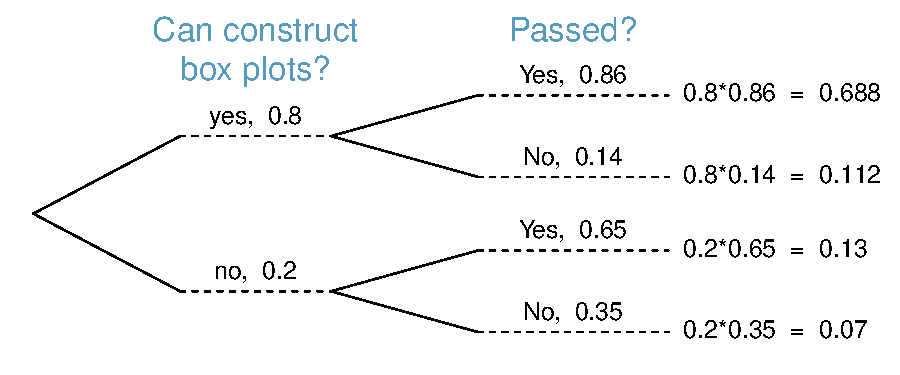
\includegraphics[width=60mm]{ch_probability/figures/eoce/tree_drawing_box_plots/tree_drawing_box_plots} \\
(b)~0.84}


\textC{\end{multicols}
\newpage
\begin{multicols}{2}}


% 23

\eocesol{0.8247. \\
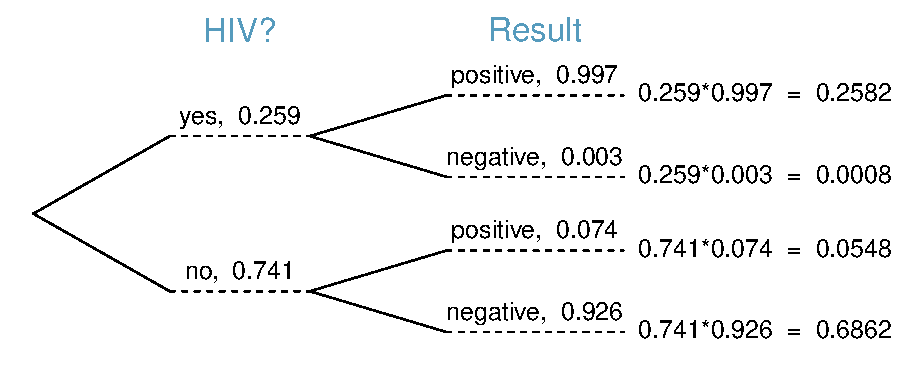
\includegraphics[width=60mm]{ch_probability/figures/eoce/tree_hiv_swaziland/tree_hiv_swaziland.pdf}}

% 25

\eocesol{0.0714. Even when a patient tests positive for lupus, there is only a 7.14\%
chance that he actually has lupus. House may be right.
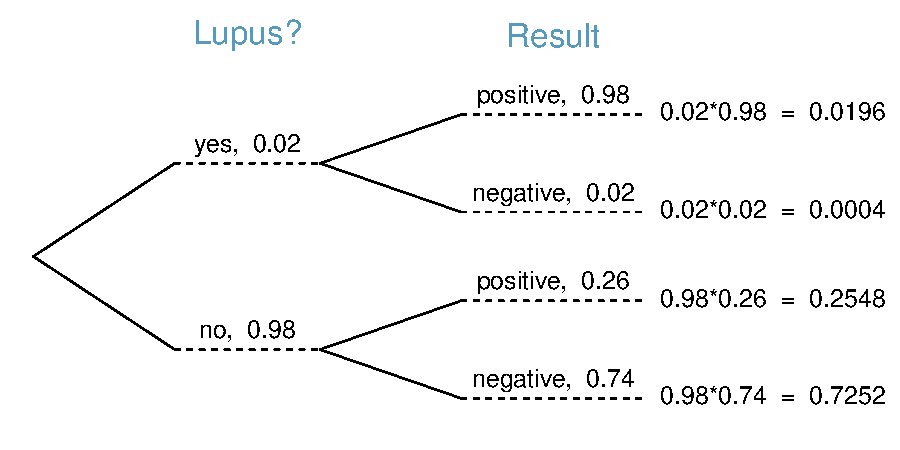
\includegraphics[width=60mm]{ch_probability/figures/eoce/tree_lupus/tree_lupus.pdf}}

% 27

\eocesol{(a)~0.3.
(b)~0.3.
(c)~0.3.
(d)~$0.3\times0.3=0.09$.
(e)~Yes, the population that is being sampled from is identical in each draw.}

% 29

\eocesol{(a)~$2/9 \approx 0.22$.
(b)~$3/9 \approx 0.33$.
(c)~$\frac{3}{10} \times \frac{2}{9} \approx 0.067$.
(d)~No, e.g. in this exercise, removing one chip meaningfully
changes the probability of what might be drawn next.}

% 31

\eocesol{$P(^1$leggings, $^2$jeans, $^3$jeans$) = \frac{5}{24} \times \frac{7}{23} \times \frac{6}{22} = 0.0173$. However, the person with leggings could have come 2nd or 3rd, and these each have this same probability, so $3 \times 0.0173 = 0.0519$.}

% 33

\eocesol{(a)~13.
(b)~No, these 27 students are not a random sample from the university's student
population. For example, it might be argued that the proportion of smokers among
students who go to the gym at 9 am on a Saturday morning would be lower than the
proportion of smokers in the university as a whole.}

% 35

\eocesol{(a)~E(X) = 3.59. SD(X) = 9.64.
(b)~E(X) = -1.41. SD(X) = 9.64.
(c)~No, the expected net profit is negative, so on average you expect to lose money.}

% 37

\eocesol{5\% increase in value.}

% 39

\eocesol{E = -0.0526. SD = 0.9986.}

% 41

\eocesol{(a)~E = \$3.90. SD = \$0.34. \\
(b)~E = \$27.30. SD = \$0.89.}

% 43

\eocesol{Approximate answers are OK. \\
(a)~$(29+32)/144 = 0.42$.
(b)~$21/144 = 0.15$.
(c)~$(26+12+15)/144 = 0.37$.}



%_______________
\end{multicols}
